\documentclass[12pt,a4paper]{article}
\usepackage[T1]{fontenc}
\usepackage[utf8]{inputenc}
\renewcommand{\familydefault}{\sfdefault}
\usepackage{graphicx}
\usepackage{verbatim}
\usepackage{float}
\usepackage{tikz}
\usepackage{pgfplots}
\usepackage{listings}
\usepackage{datetime2}
\usepackage{booktabs}
\pgfplotsset{compat=1.16}
\restylefloat{table}
\graphicspath{{reportImages/}}


\AtBeginDocument{\let\today\DTMNow}
\author{Vili Lipo, 014814253}
\title{Code Generation Project 2020: Mini-Pascal Compiler Documentation}
\begin{document}
\maketitle{}
\section{Introduction}

Few months before the world seemed like a very different place than now and I
decided that it would be a good time to learn the Rust Programming Language
while doing this project. Well life happened and it was not that great of an
idea. Despite all of that here I present to you my implementation of Mini-Pascal
written in Rust and it produces simplified C-code.

I was learning Rust while I was doing this project, so  it took me longer
than I thought to implement the features. That is why, I unfortunately did not
have time to implement "var"-parameters. Otherwise I think that
the compiler is quite feature-complete and as Rust enforces safety in many
ways I think that it has quite robust error handling too.

I also did some quite basic rookie mistakes while doing this project, like
almost finishing it completely, before I realized that the my AST-struture is
not idiomatic Rust at all, and then I reimplemented the whole parser and
compiler back-end to use the new AST.  This was very time consuming as I was
experimenting with different AST-structures with a compiler that had everything
but subroutines implemented.  I should have implemented only like integer
expressions and then experimented with different data structures.

In the end I am quite happy with the final data-structures, even though those
still ended up making the semantical analysis part of my program very verbose.
The whole project is over 4700 lines long and, I hope that it is not too
overbearing to read, and I fully recognize that no one would consider the
src/typefolder.rs to be clean code.

\section{Architecture}
The architecture of this compiler mostly follows the directions
given in the lecture materials, but instead of visiting and mutating
one AST structures, there is two distinct structures. The semantic
analysis produces the TypedAst structure, that is then
processed by the CodeGenVisitor.

\begin{figure}
  \caption{Uml of the Architecture}
  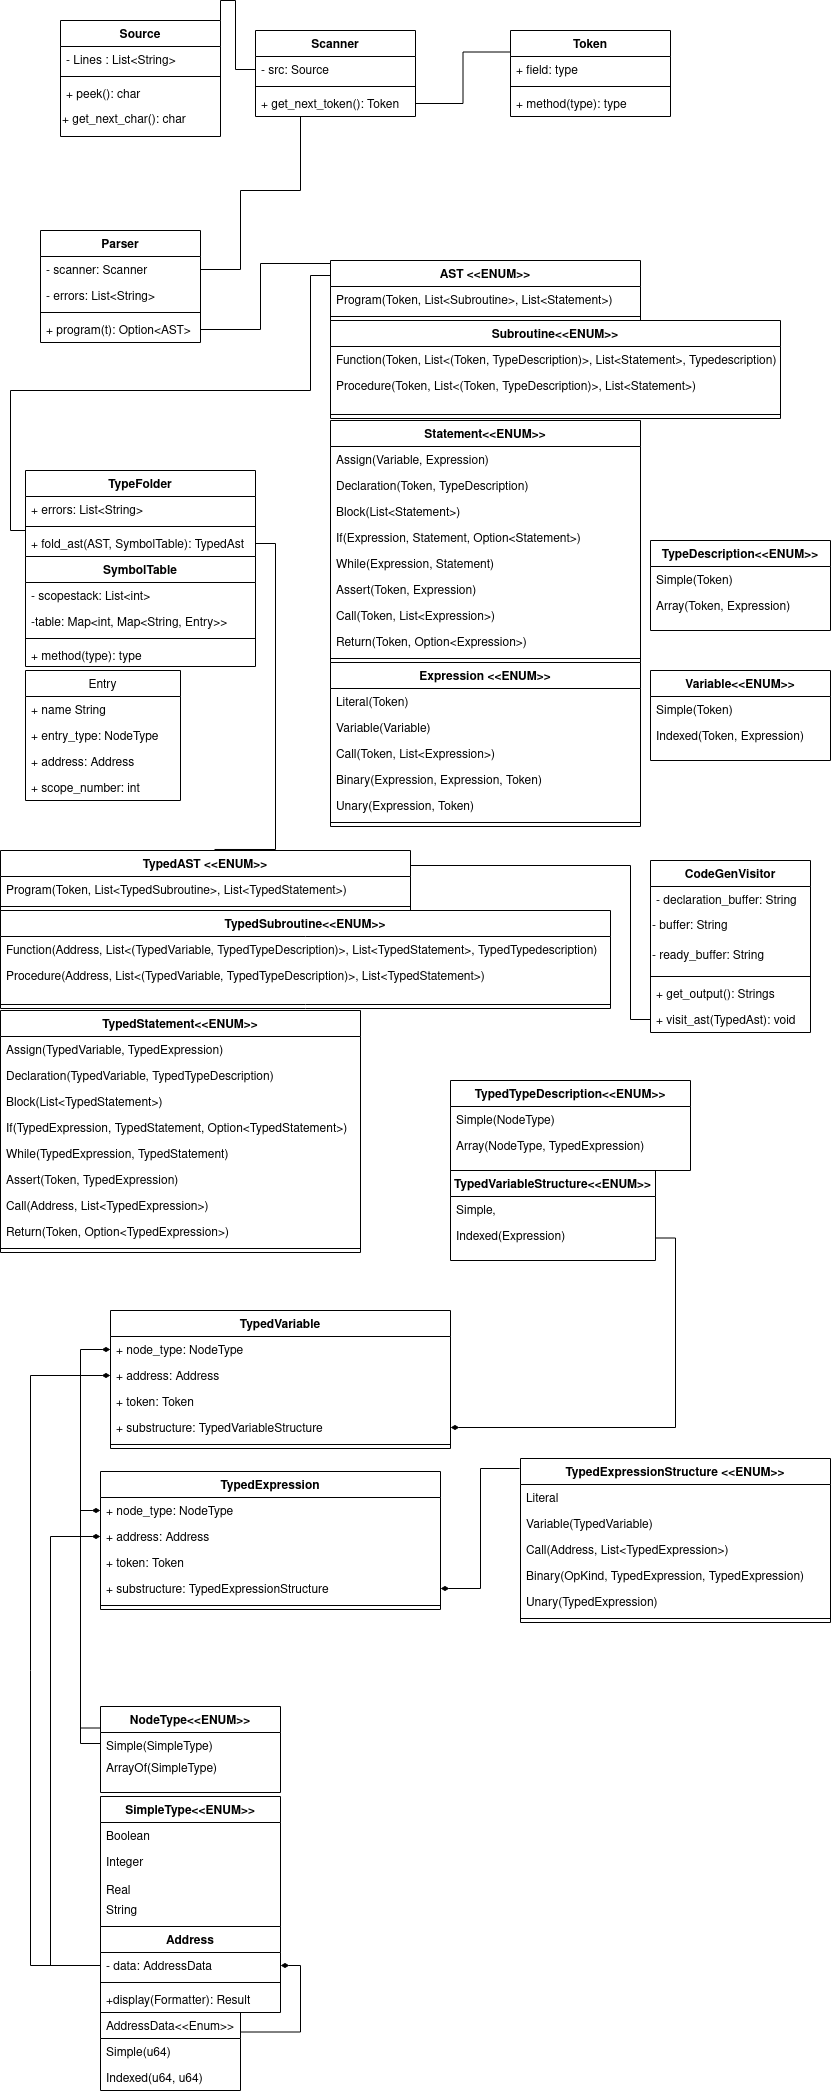
\includegraphics[scale=0.3]{ast}
\end{figure}

\section{Instructions and testing}

To build the application on Linux platform
the Rust toolchain must be installed. Then the application can be run with
\texttt{cargo run examples/test.minipascal target/test.c}. Alternatively
it can be built with \texttt{cargo build} and then the binary is
\texttt{target/debug/mini-pascal-compiler}. The test inputs
are in the folder \texttt{examples}.

\section{Mini-Pascal token patterns}
\begin{figure}
  \caption{Token patterns}\label{token_patterns}
\begin{verbatim}
<integer> ::= <digit>*
<real> ::= <digit>*\.<digit>*
<real> ::= <digit>*\.<digit>*e^<digit>*
<string_literal> ::= "[^"]*" 
<identifier> = ([a-z] | [A-Z])([a-z] | [A-Z] | _ | [0-9])*
<operator> ::= + | - | / | * | < | > | <> | <= | >=
<operator> :== and | or | not
<eof> ::=
<keyword> ::= var | if | then | else | of 
<keyword> ::= while | do | begin | end | array
<keyword> ::= procedure | function | assert | return
\end{verbatim}
\end{figure}

The token patterns can be observed in figure~\ref{token_patterns}.
Semicolons, brackets and braces have special meanings but those are
not grouped in any way so I did not list them in the regular expressions.
Nevertheless those are recognized by the scanner as tokens. Scanner
does not give any special attention to predefined identifiers.

\section{Context free grammar and techniques used to solve any problems}
\begin{figure}
\caption{Context free grammar}\label{cfg}
\begin{verbatim}
<program> ::= "program"<id>";" {<procedure> | <function>}<block>"."
<procedure> ::= "procedure" <id>"("<parameters>")"";"<block>";"
<function> ::= "function" <id>"("<parameters>")"":"<type>";"<block>";"
<var-declaration> ::= "var"<id>{"," <id>} ":" <type>
<parameters> ::= ["var"]<id> ":" <type> { "," ["var"]<id> ":" <type> }
                | <empty>
<type> ::= <simple type> | <array type>
<simple type> ::= <type id>
<array type> ::= "array" "["[<expr>]"]" "of" <simple type>
<block> ::= "begin" <statement> {";"<statement>} [";"] "end"
<statement> ::= <simple statement>
                | <structured statement>
                | <var-declaration>
<simple statement> ::= <assignment_or_call> | <return statement>
<assignment_or_call> ::= <call_or_variable> (":=" <expr> | <empty>)
<arguments> ::= <expr> {"," expr } | <empty>
<return statement> ::= "return" [<expr>]
<structured statement> ::= <block> | <if statement> | <while statement>
<if statement> :== "if" <expr> "then" <statement> [ "else" <statement>"]
<while statement> ::= "while" <expr> "do" <statement>
<expr> ::= <simple expr> [ <relational operator> <simple expr> ]
<simple expr> ::= [<sign>] <term> { <adding operator> <term> }
<term> ::= <factor> {<multiplying operator> <factor>}
<factor> ::= <call_or_variable> | <literal> 
<factor> ::= "("<expr>")" | "not" <factor>
<call_or_variable> ::= <id><call_or_variable_tail>
<call_or_variable_tail> ::= [<expression>]
                           | (<parameters>)
                           | ".""size"
                           | <empty> 
\end{verbatim}
\end{figure}

The Mini-Pascal context free grammar can be observed in figure~\ref{cfg}.
Here a call or variable construction is created to solve the violation
of LL (1) rule. Now as the language syntax does not allow
to assign a value to a call, in the parsing function the return type
of call or variable is checked and based on that we see if
the assign can be constructed. If a call is not followed by ":=" 
a call statement is returned. So no actual backtracking is used,
this is like using LR parsing for a one part of the syntax.
In factor this does not create any issues as all of the
variants of call or variable are legal variants of factor.

The parser does not recognize writeln or read as statements.
Those are parsed as regular calls. Those are
recognized by the TypeFolder, so that user might redefine
the identifier if he/she wishes to do so.

\section{AST-specifications}

For my first AST-produced by the parser I think the source code is the most
easy way to explain it. I think that it is better than UML, as Rust provides
very good tools for this kind of structure. The code is in
figure~\ref{ast_source}.  The AST is represented as enums with different
variants for each structure. We see that AST-contains a variant program that
has three parts, Token produced by the scanner, a list of subroutines and a
list of statements being the main block. Then Subroutine is an enum with two
variants function and procedure. Both of them have token, and parameters that
are a list of tuples that have a token for the name and a type-description enum
for the type construction. Functions have one additional type-description for
the function output type.

In Rust to support recursive enum structures, the recursive definitions must
be wrapped in Box objects. This is used in the Statement and Expression enums.
In statement the If variant has \texttt{Option<Box<Statement> >} as its third field
as the else branch may or may not be present.

\begin{figure}
  \caption{AST source code}\label{ast_source}
\begin{lstlisting}
pub enum AST {
    Program(Token, Vec<Subroutine>, Vec<Statement>),
}

pub enum Subroutine {
    Function(
        Token,
        Vec<(Token, TypeDescription)>,
        Vec<Statement>,
        TypeDescription,
    ),
    Procedure(Token, Vec<(Token, TypeDescription)>, Vec<Statement>),
}

pub enum Statement {
    Assign(Box<Variable>, Expression),
    Declaration(Token, TypeDescription),
    Block(Vec<Statement>),
    If(Expression, Box<Statement>, Option<Box<Statement>>),
    While(Expression, Box<Statement>),
    Assert(Token, Expression),
    Call(Token, Vec<Expression>),
    Return(Token, Option<Expression>),
}

pub enum Expression {
    Literal(Token),
    Variable(Box<Variable>),
    Binary(Box<Expression>, Box<Expression>, Token),
    Unary(Box<Expression>, Token),
    Call(Token, Vec<Expression>),
}

pub enum TypeDescription {
    Simple(Token),
    Array(Token, Expression),
}

pub enum Variable {
    Indexed(Token, Expression),
    Simple(Token),
}
\end{lstlisting}
\end{figure}

Instead of decorating this structure by mutating it, the TypeFolder object
folds this AST to TypedAst structure that contains the type-infomation and
addressing information needed by the code generation. TypeFolder does most of
the heavy lifting in the backend of this compiler.  As a result the
CodeGeneration visitor does not even need to access the symboltable or mutate
the created TypedAst structure.

Using the folder pattern instead of the visitor pattern made the TypeFolder
more verbose than its visitor counterpart. I implemented most of the
application using a mutable data-structure first, before I refactored it to use
the new data-structure. This is because there is quite a lot of code handling
the building of the new typed nodes. Also compared to some more object oriented
languages polymorphism in Rust felt a bit awkward and so this enum structure
warrants use of large match-operator case switches in the visitor and folder
code. The code base is quite verbose for that reason. The benefits of this are
the that code-generation part can have very straightforward control-flow and
still be completely safe.

In the TypedAst datastructure the TypedExpression is made in to a struct,
that holds all of the important information. In its field
substructure it contains a value of enum TypedExpressionStrucure that
again models the different types of Expressions with types.
This same idiom is also applied to typed variables. The TypedAst structure is
then just visited by the CodeGeneration visitor to produce the output
C-code.

In TypedAst the Read and Write statement variants are introduced.
The TypeFolder can determine with its symbol table if user
has redefined the identifier to mean some other value, or
if it still means the special statement.

\section{Implementation level decisions}

My implementation of Mini-Pascal has static scope, since it felt bit more
natural in the unlimited register machine idiom.  If I had  modelled some
runtime stack, then dynamic scope might have been a good alternative.

Var-parameters are not implemented to the final version due to lack of time.
So instead arrays are passed as references to subroutines.  And other types as
values. Strings are char-pointers in my compiled C, but due to every string
concatenation allocating a new memory section it does not mutate the existing
string. This is somewhat similar to how simple and
complex types work in Java.

Strings have maximum length of 512 characters, but for literals only
the needed amount of memory is allocated. There is no garbage collection
whatsoever.

Recursive calls work. A subroutine can call subroutines that were declared
before it but not the ones that are declared after it.

Predefined identifiers are added to the symbol table when it is created.  There
entries for type identifiers, special subroutines and predefined values are
added to top scope. Then in TypeFolder if a user covers any of these names in
lower scopes the new entries will appear first in a lookup operation.
The change to declare the subroutines before folding their bodies is not trivial,
but doable.

Booleans are printed as integers 0 meaning false and 1 true.
This could be fixed by extending the runtime.


\section{Semantic analysis}

The TypeFolder does a large amount of semantic analysis.  It type checks all
expressions, assignments and calls.  Basically for all expressions except the
relational ones, if the operator is applicable to the arguments and the
arguments are of the same type, then the expression has the same type as the
arguments. For the relational operations the sides are checked in the same way
but the type of the expression is boolean.

For statements, in if, while and assert statements the conditions are checked to 
be of the type boolean.

In assign statements the left hand side variable
must have matching type to the right hand side expression.
For declarations it is checked that the variable is not declared twice
in same scope. Then the type identifier is checked to be a correct type
identifier in the symboltable. 
In declarations the array size expression is checked to be of the type integer.
Same goes for array variable indexes.

For read statements it is checked that all of its arguments are
variables. Write statement accepts all arguments.

For functions the TypeFolder checks that a function has a return statement that
returns a value of correct type.

Calls are checked so that procedure calls can only
exist as statements and function calls can only exist as
expressions. It is also checked that the argument types match
the parameter types.


\begin{figure}
\caption{Complete list of semantical checks}
\begin{enumerate}
  \item Subroutines
    \begin{enumerate}
      \item Subroutine must return a correct type
    \end{enumerate}
  \item Expressions
    \begin{enumerate}
      \item Both sides have the same type
      \item Operator is applicable to the type
    \end{enumerate}
  \item Variables
    \begin{enumerate}
      \item Variable is declared before use
      \item Variable is not declared twice in same scope
      \item Array variable index must be integer
    \end{enumerate}
  \item Type identifiers 
    \begin{enumerate}
      \item Identifier used as a type must be a valid type
      \item Array Type length expression must be integer
    \end{enumerate}
  \item Statements
    \begin{enumerate}
      \item If condition must be a boolean
      \item While condition must be a boolean
      \item Assert condition must be a boolean
      \item Assignment types must match, and the variable must be declared before assignment.
      \item Call
        \begin{enumerate}
          \item Only identifiers that are either functions or procedures can be called
          \item Argument types must match the parameter types for the subroutine
          \item Only procedure calls are accepted as statements, and function calls as expressions
        \end{enumerate}
  \item Read statement parameters must be variables

    \end{enumerate}

\end{enumerate}

\end{figure}


\section{Major problems and solutions}

I explained how I solved the LL (1) violations in the third section.  In
addition to the biggest issues was how to efficiently model the AST without
redundant code in the data structure or the visitors and folders.  I found that
implementing static scope using the lecture materials was quite straight
forward.  Maybe attending the ``Ohjelmointikielten Periaatteet'' course helped me
in that task, as scoping was one of the primary study interests on that course.

First I was bit unsure how using goto for flow-control would affect the
code-generation.  Mostly I worried how to ensure that variables are declared
only once. Then I designed the three buffer system, where the code is generated
to three separate string buffers. The first is for declarations, and second is
for the main body of the code.  Then when a subroutine or main block is
complete the both of the buffers are pushed to the ready buffer the
declarations first. Using this method the gotos can not cause duplicate
declarations in C-runtime. This actually reminded me from a code style rule
from my C-programming course in Lappeenranta University Of Technology, where
the lecturer demanded that all variables are declared at the start of a
function. Now it clicked that in that way the code would resemble the assembly
generated by C-compiler and thats why the lecturer preferred to have it that
way.

The specification for I/O-operations was a positive suprise to me, as it was
easy to match the desired behaviour using C-standard library functions
`printf' and `scanf'.

Arrays were a bit difficult to figure out, as the size is determined in runtime
C, so dynamic memory management had to be used. I decided to save the size for
every array in a variable called \texttt{\{address\}\_size}.  This variable is
set the value of the size expression at the array declaration, and then the
\texttt{.size} function was trivial to implement.

My enum-based data-structure essentially made me use a lot of \texttt{match}
statements in a switch-like fashion in the code base. Many would argue that
this is not clean code at all, and that the switches should neatly contained in
some factory that produces some polymorphic objects that would behave nicely
during code generation.  I found doing that too difficult as I am a Rust
novice. I don't know if such polymorphic structure would even be idiomatic Rust
as the Rust compiler written in Rust uses these enum-based structures in its
own abstract syntax model. As a whole I found working with Rust to be
challenging but still very rewarding.

The memory management in the generated code is abysmal. No attempt at garbage
collection is done and the string concatenation is especially offending in this
category, as every step concatenation reserves a fresh section for the result.
If this is done in a loop every iteration reserves more memory that is 
never freed. This could be fixed by rewriting assignment for strings.
Now the char pointer of the result is set as the value of the left hand
side variable. If \texttt{strcpy} would be used to assign a value, then
the expressions would not need to reserve new memory every time those are run.


\section{Error handling strategies}

For error handling I heavily utilize the Rust Option-enum, that
has variants Some(<T>), and None. So if a parsing method
is successful it returns Some(expression) for example.
If it fails it returns None. Then the caller can check that
what variant it received by using this if let statement: 
\begin{verbatim}
if let Some(expression) = self.expression() {
  // do something with expression
}
\end{verbatim}
or the match statement:
\begin{verbatim}
match self.expression() {
  Some(expression) => {
      // do somethign with expression
      },
  None => println("Could not parse expression!")
}
\end{verbatim}

This success based control-flow is heavily used in the parser, and TypeFolder.
This might have been the case that I found the new ``Silver bullet'' of safe code
and overused it so much that it actually falls to the anti-pattern category.

In the parser I only create a error message from the lowest level where the
error occurs.  So when a parsing-method calls a another parsing-method that
returns None the none is just forwarded upwards. If the error is the result
of expecting a certain token and something else appears, then an error message
is added to ``parser.errors'' and None is returned. This usually
leads to re-synchronization at statement level. Especially bad 

If the syntax is so broken that the parser can not procedure a sensible
AST-from it naturally no semantic analysis can be done.

The TypeFolder has quite similar approach to error handling. So if a folding
method cannot produce a correctly typed node, it returns None that is passed along,
usually to statement level. At the source of the problem an error message is
appended to TypeFolders error list.

There is minimal error handling in CodeGenVisitor, as the TypedFolder takes
care that the TypedAst-passed to CodeGenVisitor is safe to compile.  Trying to
write an array makes \texttt{printf} format string to be ``Error array printing
not implemented''. In addition to that if the visitor fails to read a C-runtime
file an error message is printed. This is the extent of error handling in the
CodeGeneration visitor.

\section{Work hour log}
\begin{center}
  \begin{tabular}{l l l}
    \bottomrule
    Date & Duration & Task \\
    23.3 & 3h & Creating module Source \\
    \bottomrule
    23.3 & 1h & Initial testing of Source \\
    \bottomrule
    24.3 & 4h & Creating Scanner \\
    \bottomrule
    24.3 & 2h & Initial testing of Scanner \\
    \bottomrule
    26.3 & 5h & Initial recursive parser with just ints and main block\\
    \bottomrule
    26.3 & 3h & Initial AST \\
    \bottomrule
    27.3 & 1h & PrintVisitor \\
    \bottomrule
    30.3 & 8h & Writing SemanticVisitor and CodeGeneration for ints\\
    \bottomrule
    31.3 & 4h & Adding booleans and reals \\
    \bottomrule
    3.4 - 5.5 & Focusing on other courses \\
    \bottomrule
    5.5 & 4h & Adding strings \\
    \bottomrule
    6.5 & 3h & Adding actually simple arrays \\
    \bottomrule
    8.5 & 2h & Adding string arrays \\
    \bottomrule
    10.5 & 2h & Implementing size \\
    \bottomrule
    11.5 & 4h & assert and parameters \\
    \bottomrule
    13.5 & 3h & Parsing subroutines \\
    \bottomrule
    14.5 & 3h & Refactoring AST and parser \\
    \bottomrule
    15.5 & 2h & Refactoring AST and printvisitor\\
    \bottomrule
    15.5 & 2h & SemanticVisitor to be TypeFolder\\
    \bottomrule
    16.5 & 10h & Refactoring AST and implementing TypeFolder.\\
    \bottomrule
    17.5 & 8h & Refactoring AST, Typefolder and CodeGeneration.\\
    \bottomrule
    18.5 & 1h & Reimplementing code generation\\
    \bottomrule
    18.5 & 1h & Created Address data-structure\\
    \bottomrule
    19.5 & 2h & Reimplementing code generation\\
    \bottomrule
    21.5 & 8h & Parsing parameters, Subroutine semantic analysis \\
    \bottomrule
    22.5 & 3h & Subroutine semantic analysis, parameter analysis\\
    \bottomrule
    23.5 & 2h & Writing report\\
    \bottomrule
    23.5 & 6h & Implementation of subroutine code generation, testing\\
    \bottomrule
    25.6 & 6h & Wrapping up. \\
    \bottomrule
    Total & 103h & Total
  \end{tabular}
\end{center}


\end{document}
